% tirlnx01 - Materiaal om het keuzevak Linux te geven 
% op de Hogeschool Rotterdam.
% Copyright (C) 2010 - 2011  Paul Sohier, Kevin van der Vlist
%
% This program is free software: you can redistribute it and/or modify
% it under the terms of the GNU General Public License as published by
% the Free Software Foundation, either version 3 of the License, or
% (at your option) any later version.
%
% This program is distributed in the hope that it will be useful,
% but WITHOUT ANY WARRANTY; without even the implied warranty of
% MERCHANTABILITY or FITNESS FOR A PARTICULAR PURPOSE.  See the
% GNU General Public License for more details.
%
% You should have received a copy of the GNU General Public License
% along with this program.  If not, see <http://www.gnu.org/licenses/>.
%
% Kevin van der Vlist - kevin@kevinvandervlist.nl
% Paul Sohier - paul@paulsohier.nl

\documentclass{beamer}

\mode<presentation>

\usepackage[dutch]{babel}
\usepackage{listings}
%\usepackage{beamerthemesplit}

\lstset{ %
  language=bash,                % choose the language of the code
  basicstyle=\footnotesize,       % the size of the fonts that are used for the code
  numbers=left,                   % where to put the line-numbers
  numberstyle=\footnotesize,      % the size of the fonts that are used for the line-numbers
  numbersep=5pt,                  % how far the line-numbers are from the code
  showspaces=false,               % show spaces adding particular underscores
  showstringspaces=false,         % underline spaces within strings
  showtabs=false,                 % show tabs within strings adding particular underscores
  frame=lr,	                % adds left and right lines
  tabsize=2,	                % sets default tabsize to 2 spaces
  captionpos=b,                   % sets the caption-position to bottom
  breaklines=true,                % sets automatic line breaking
  breakatwhitespace=false,        % sets if automatic breaks should only happen at whitespace
%  escapeinside={\%*}{*)},         % if you want to add a comment within your code
  morekeywords={*,...}            % if you want to add more keywords to the set
}

\usetheme{Berlin}
\useinnertheme{rounded}
\usecolortheme{rose}
\setbeamertemplate{navigation symbols}{} 

\title{Keuzevak Linux - Week 4}
\author{Paul Sohier \and Kevin van der Vlist}
\institute{Versie $1.0$}
\date{\today}

\begin{document}

\begin{frame}
  \titlepage
\end{frame} 

\begin{frame}
  \frametitle{Inhoud}
  \tableofcontents
\end{frame}

\section{Device files}

\begin{frame}
  \frametitle{Device files - Algemeen}
  \begin{itemize}
  \item<1-> interfaces op filesystem naar hardware of software
  \item<2-> naamgeving komt uit de kernel
  \item<3-> \texttt{/dev/device}
  \item<4-> character devices
  \item<5-> block devices
  \end{itemize}
\end{frame}

\begin{frame}
  \frametitle{Device files - character devices}
  \begin{itemize}
  \item<1-> simpele lees-, en schrijf operaties
  \item<2-> interfaced door driver
  \item<3-> printers, muizen, terminals, \ldots
  \end{itemize}
\end{frame}

\begin{frame}
  \frametitle{Device files - block devices}
  \begin{itemize}
  \item<1-> adresseerbare data blokken
  \item<2-> vaak directe toegang
  \item<3-> geheugen, schijven, \ldots
  \end{itemize}
\end{frame}

\begin{frame}
  \frametitle{Device files - handige files}
  \begin{itemize}
  \item<1-> null
  \item<2-> random % Blocking, hq rnadom
  \item<3-> urandom % Nonblocking, pseudo random
  \end{itemize}
\end{frame}

\section{Networking}

\begin{frame}
  \frametitle{Networking}
\end{frame}

\begin{frame}
  \frametitle{Networking - devices}
  \begin{itemize}
  \item<1-> \texttt{eth0}, \texttt{ath2}
  \item<2-> \texttt{lo:0}
  \end{itemize}
\end{frame}

\begin{frame}
  \frametitle{Networking - configuratie}
  \begin{itemize}
  \item<1-> frontends: \texttt{netconfig}
  \item<2-> files: \texttt{/etc/rc.d/rc.inet1.conf}
  \item<3-> \texttt{ifconfig}
  \end{itemize}
\end{frame}

\begin{frame}
  \frametitle{Networking - static HRO}
  \begin{itemize}
  \item<1-> \texttt{ifconfig eth1 145.24.222.162 netmask 255.255.255.0 up}
  \item<2-> \texttt{route add 145.24.222.253 dev eth1}
  \item<3-> \texttt{route add default gw 145.24.222.253}
  \end{itemize}
\end{frame}

\begin{frame}
  \frametitle{Networking - Remote shell}
  \begin{itemize}
  \item<1-> vroeger \texttt{rlogin} + \texttt{rsh}
  \item<2-> momenteel secure shell; \texttt{ssh}
  \item<3-> \texttt{ssh hostname.nl -l kevin -p 22}
  \end{itemize}
\end{frame}

\begin{frame}[fragile]
  \frametitle{Networking - fingerprints}
  \begin{itemize}
  \item<1-> uniek
  \item<2-> voorkomen man in the middle aanvallen
  \item<3-> 
    \begin{lstlisting}
kevin@slackbak:~$ ssh-keygen -l
Enter file in which the key is (/home/kevin/.ssh/id_rsa): /etc/ssh/ssh_host_rsa_key  
2048 0e:35:8e:be:6a:61:f0:cc:b1:ef:fe:a6:7f:f6:a5:df /etc/ssh/ssh_host_rsa_key.pub (RSA)
    \end{lstlisting}%$
  \end{itemize}
\end{frame}

\section{X.org}

\begin{frame}
  \frametitle{X.org}
\end{frame}

\begin{frame}
  \frametitle{X.org - algemeen}
  \begin{itemize}
  \item<1-> faciliteert grafische mogelijkheden
  \item<2-> client - server model
  \end{itemize}
\end{frame}

\begin{frame}
  \frametitle{X.org - overzicht}
  \begin{figure}[h]
    \begin{center}
      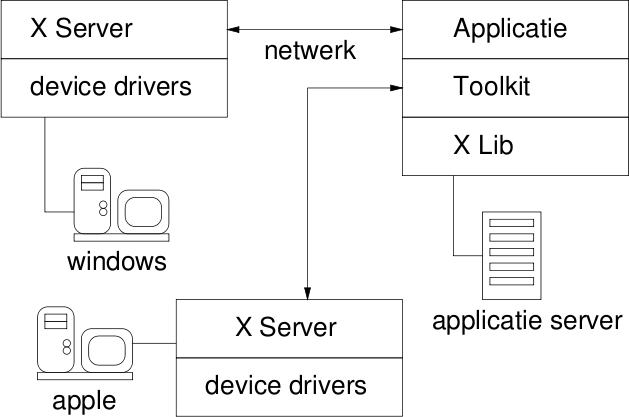
\includegraphics[scale=0.3]{../../dictaat/images/xserver2}
    \end{center}
    \caption{X client/server overzicht}
    \label{fig:xs2}
  \end{figure}
\end{frame}

\begin{frame}
  \frametitle{X.org - remote X}
  \begin{itemize}
  \item<1-> gebruikt client - server model
  \item<2-> \texttt{ssh -XY -l kevin hostname.nl}
  \item<3-> localhost: X server
  \item<3-> hostname.nl: X client
  \end{itemize}
\end{frame}

\begin{frame}
  \frametitle{X.org - window managers}
  \begin{itemize}
  \item<1-> tussen gebruiker en X
  \item<2-> flexibel
  \item<3-> onderdeel desktop environment
  \item<4-> \texttt{Kwin}, \texttt{Metacity}, \texttt{Fluxbox}, \texttt{Awesome}, \ldots
  \end{itemize}
\end{frame}

\end{document}
